\documentclass[xetex,aspectratio=43]{beamer}

\usepackage{res/lections}

\preamble

\title[Шины и периферийные устройства]{Шины, периферийные устройства, ввод/вывод и прерывания}

\begin{document}

\titleslide

\tocslide

\section{Шины и периферийные устройства}

\subsection{Периферийные устройства и контроллеры}

\begin{frame}{Вспоминаем: архитектура фон Неймана}
	\begin{figure}
		\includesvg[height=0.5\textheight]{img/03.Von_Neumann_System_Bus_rus.svg}
	\end{figure}
\end{frame}

\begin{frame}{Оборудование и ПО}
	\begin{itemize}
		\item
		\defn{Контроллер}{устройство в составе ЭВМ, обеспечивающее связь
			системной шины с внешним устройством}

		\begin{itemize}
			\item
			Например, контроллер жёсткого диска, контроллер порта USB
		\end{itemize}
		\item
		\defn{Драйвер устройства}{ПО, предоставляемое производителем
			устройства или ОС}

		\begin{itemize}
			\item
			Реализует низкоуровневые операции работы с устройством
			\item
			Позволяет абстрагироваться от модели оборудования.
			Например: для прикладного ПО и ОС все принтеры «одинаковые», т.к. разные драйвера принтеров реализует один и тот же стандартный программный интерфейс
		\end{itemize}
	\end{itemize}
\end{frame}

\begin{frame}[fragile]{Взаимодействие контроллера с ЦП}
	Устройство соединено с системной шиной

	\begin{itemize}
		\tightlist
		\item
		реагирует на сигнал шины управления «работа с устройствами»
		\item
		проверяет, совпадает ли его идентификатор со значением на шине адреса
		\item
		по команде на шине управления может прочитать данные с шины данных или записать на неё
		\item
		может генерировать \emph{аппаратные прерывания} (позже), сообщая об этом через шину управления
	\end{itemize}

	\defn{Адрес устройства}{его идентификатор. Не является адресом в смысле
		адреса данных в ОЗУ, но передаётся по шине адреса}

	\begin{itemize}
		\tightlist
		\item
		Соединение устройства с шиной --- порт (port)
		\item
		Инструкция записи в порт --- \texttt{out\ адрес,\ регистр}
		\item
		Инструкция чтения из порта --- \texttt{in\ адрес,\ регистр}
	\end{itemize}

	\defn{Порт}{аппаратная и программная абстракция: механизм
		сопряжения контроллера устройства с системной шиной и механизм
		программного обращения к контроллеру}

	Обычно говорят «номер порта» или «адрес порта». У устройства может быть
	и несколько портов.
\end{frame}

\begin{frame}{Внешние устройства и системная шина}
    \begin{figure}
    \includesvg[height=0.5\textheight]{img/03.Von_Neumann_Multiple_Peripherals.svg}
\end{figure}
\end{frame}

\begin{frame}{Немного истории}
	\begin{itemize}
		\tightlist
		\item
		В ранних и простых ЭВМ типичным было подключение устройств
		непосредственно к системной шине. Поэтому «порт» --- разъём на корпусе
		и «порт» --- способ доступа к устройству были практически синонимами

		\begin{itemize}
			\tightlist
			\item
			Пример: ZX Spectrum
			\href{https://en.wikipedia.org/wiki/ZX_Interface_1}{Interface 1} ---
			фактически это был контроллер
		\end{itemize}
		\item
		Сейчас разъём на корпусе --- обычно способ присоединить устройство к
		контроллеру в ПК, а в устройстве «говорить» с контроллером в ПК будет
		ответный контроллер

		\begin{itemize}
			\tightlist
			\item
			Пример: универсальный USB-контроллер в ПК и USB-клавиатура со своим
			внутренним контроллером
		\end{itemize}
	\end{itemize}
\end{frame}


\section{Прерывания}

\subsection{Основы аппаратных прерываний}

\begin{frame}{Ситуации}
	\begin{block}{«Системные горячие клавиши»}
		Ctrl+Alt+Del на PC:

		\begin{itemize}
			\tightlist
			\item
			немедленная перезагрузка (DOS)
			\item
			завершение и перезагрузка (Linux)
			\item
			вызова системного меню (Windows)
		\end{itemize}

		При этом ни ОС, ни, тем более, пользовательская программа, не проверяют всё время: не нажали ли Ctrl+Alt+Del?

		\pause
		\begin{itemize}
			\item
			Значит прерывание по Ctrl+Alt+Del на USB-клавиатуре генерируется
			программно драйвером клавиатуры
		\end{itemize}

	\end{block}

	\pause

	\begin{block}{Мышь}
		\begin{itemize}
			\tightlist
			\item
			Ни прикладные программы, ни ОС не опрашивают мышь постоянно
			\item
			Тем не менее «что-то» реагирует на движение мыши и отображает на
			экране движущийся указатель
		\end{itemize}
	\end{block}
\end{frame}

\begin{frame}
	\begin{block}{Аппаратное прерывание}
		\textbf{Аппаратное прерывание} --- сигнал, сообщающий ЦП о возникновении
		ситуации, требующей немедленной обработки

		\begin{itemize}
			\tightlist
			\item
			Обычно этот сигнал генерируют контроллеры внешних устройств
			\item
			Обработка ситуации выполняется программно
			\item
			Текущая выполняемая программа «не замечает» того, что процессор
			«отвлёкся», и после обработки ситуации продолжается
		\end{itemize}
	\end{block}
\end{frame}

\begin{frame}
	\begin{block}{Обработка прерываний}
		\begin{itemize}
			\tightlist
			\item
			Запускается и работает ОС

			\begin{itemize}
				\tightlist
				\item
				ОС регистрирует адреса специальных процедур --- обработчиков
				прерываний; обработчик прерывания --- часть драйвера устройства
				\item
				Прерываний от разных устройств множество (они имеют номера), адреса
				обработчиков помещаются в специальный массив в ОЗУ --- вектор
				прерываний
			\end{itemize}
			\item
			Запускается и работает прикладное ПО

			\begin{itemize}
				\tightlist
				\item
				Выполняется программа
				\item
				Получив сигнал от устройства (например, мыши), контроллер посылает
				сигнал ЦП о необходимости его обработки (проверить, на сколько
				переместили мышь, какие кнопки нажали)
				\item
				ЦП заканчивает выполнение очередной инструкции, а вместо следующей
				производит вызов процедуры --- обработчика прерывания. Эта процедура
				--- не часть прикладной программы
				\item
				После завершения обработчика прерывания продолжается выполнение
				прикладной программы
			\end{itemize}
		\end{itemize}
	\end{block}
\end{frame}

\begin{frame}{Вектор прерываний}
	\begin{figure}
		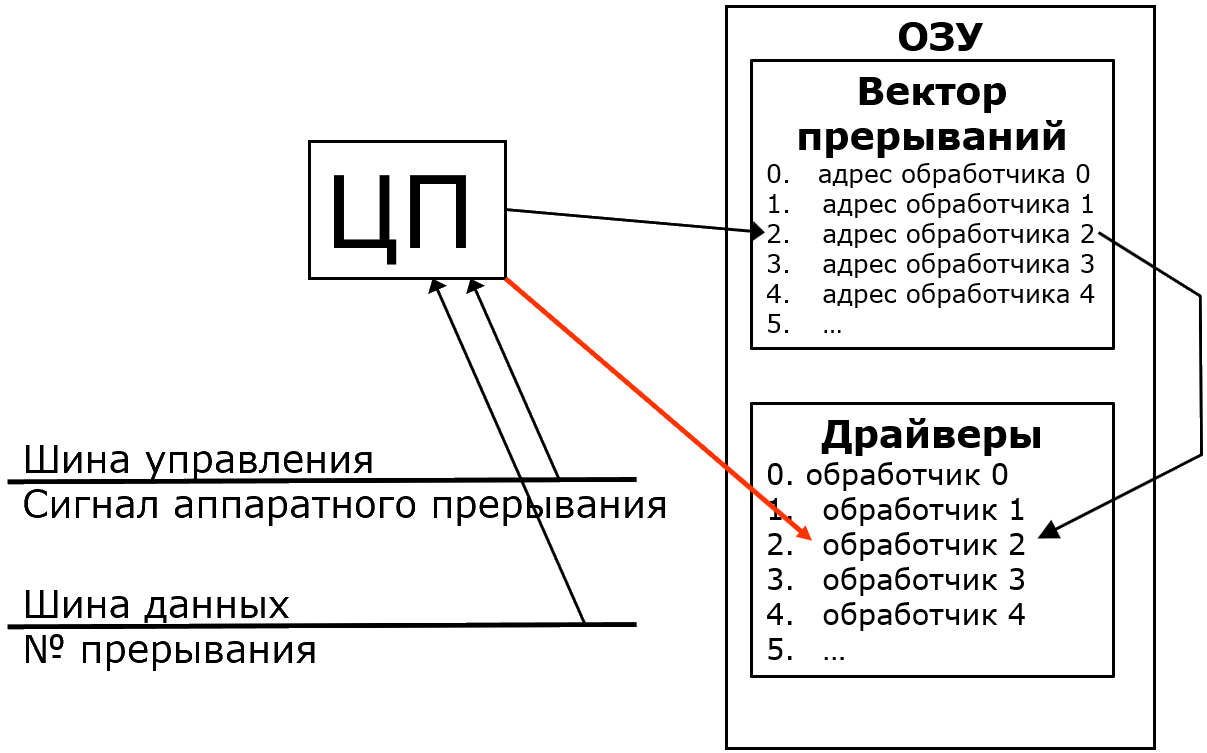
\includegraphics[height=0.75\textheight]{img/03.interrupt_vector.png}
	\end{figure}
\end{frame}

\begin{frame}{Обработка прерываний}
	\begin{figure}
		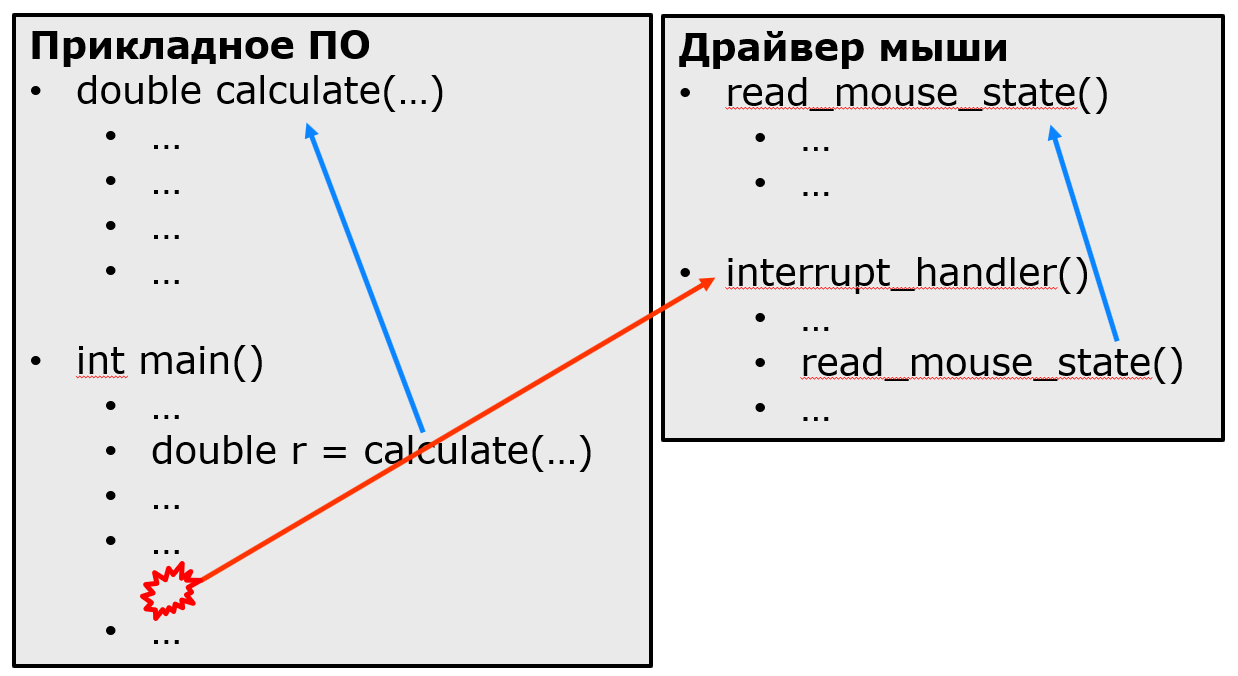
\includegraphics[height=0.7\textheight]{img/03.interrupt_invokation.png}
	\end{figure}
\end{frame}

\subsection{Другие способы использования прерываний}

\begin{frame}[fragile]{Косвенный вызов API ОС (в недавнем прошлом)}
	\begin{itemize}
		\tightlist
		\item
		Прерывание генерируется программно, на PC --- машинная команда
		\texttt{int\ \textless{}номер\textgreater{}}
		\item
		Вектор прерываний фактически хранит адреса части системных функций
		\item
		Это позволяет менять адреса системного кода, не меняя машинного кода
		пользовательских программ
	\end{itemize}

	\begin{block}{Где это использовалось?}
		\begin{itemize}
			\tightlist
			\item
			Вызов API BIOS для управления графикой (\mintinline{as}{int 10h}) и DOS
			(\mintinline{as}{int 21h})

			\begin{itemize}
				\tightlist
				\item
				Пример

				\begin{minted}[autogobble]{as}
                    mov ah, 0eh     ; function number = 0Eh : Display Character
                    mov al, '!'     ; AL = code of character to display
                    int 10h         ; call INT 10h, BIOS video service
				\end{minted}
			\end{itemize}
		\end{itemize}

		\begin{itemize}
			\tightlist
			\item
			Вызов API ядра Windows (\mintinline{as}{int 2Eh})
			\item
			Вызов API ядра Linux (\mintinline{as}{int 80h})
		\end{itemize}

		Этот способ удобный, но механизм прерываний небыстрый

		\pause
	\end{block}
\end{frame}

\begin{frame}{Вызов API ОС в наши дни}
	\begin{itemize}
		\item
		Windows и Linux используют специально разработанные инструкции
		(\mintinline{as}{syscall}, \mintinline{as}{sysenter}) и техники (vDSO). \href{https://habr.com/ru/post/347596/}{Подробнее здесь}
	\end{itemize}
\end{frame}

\begin{frame}
	\begin{block}{Обработка внутренних событий ЦП}
		Вызов драйвера виртуальной памяти, когда страница памяти выгружена или
		не проинициализирована

		\pause

		О виртуальной памяти позже

	\end{block}
\end{frame}

\section{DMA}

\subsection{DMA для высокопроизводительных устройств}

\begin{frame}
	\begin{block}{Предмет}
		Внешние устройства могут передавать значительные объёмы информации.
		Основные способы взаимодействия:

		\begin{itemize}
			\tightlist
			\item
			Чтение и запись в порты. Обмен небольшими порциями данных загружает ЦП
			\item
			Выделение контроллеру устройства области памяти и выдача команд,
			которые выполняются отложено
		\end{itemize}

		\pause

		\defn{DMA (Direct Memory Access)}{механизм прямого обмена данными
			между оперативной памятью и контроллерами устройств}

		Механизм поддерживается многими контроллерами устройств,
		предназначенными для передачи значительных объёмов данных. Для небольших данных (например, работа с системными часами) необходимости его использовать нет.
	\end{block}
\end{frame}

\begin{frame}
	\begin{block}{Сообщение о завершении операции}
		Для того чтобы сообщить о завершении операции, контроллер генерирует
		аппаратное прерывание. Обработчик прерывания находится в драйвере
		соответствующего устройства
	\end{block}
\end{frame}

\subsection{DMA для устройств реального времени}

\begin{frame}{DMA для потоковых устройств реального времени}
	А когда Sound Blaster «доиграет» фрагмент звука, он сгенерирует
	прерывание, и будет ждать, пока ЦП не выдаст ему ещё данных?..

	\pause

    \begin{figure}
    	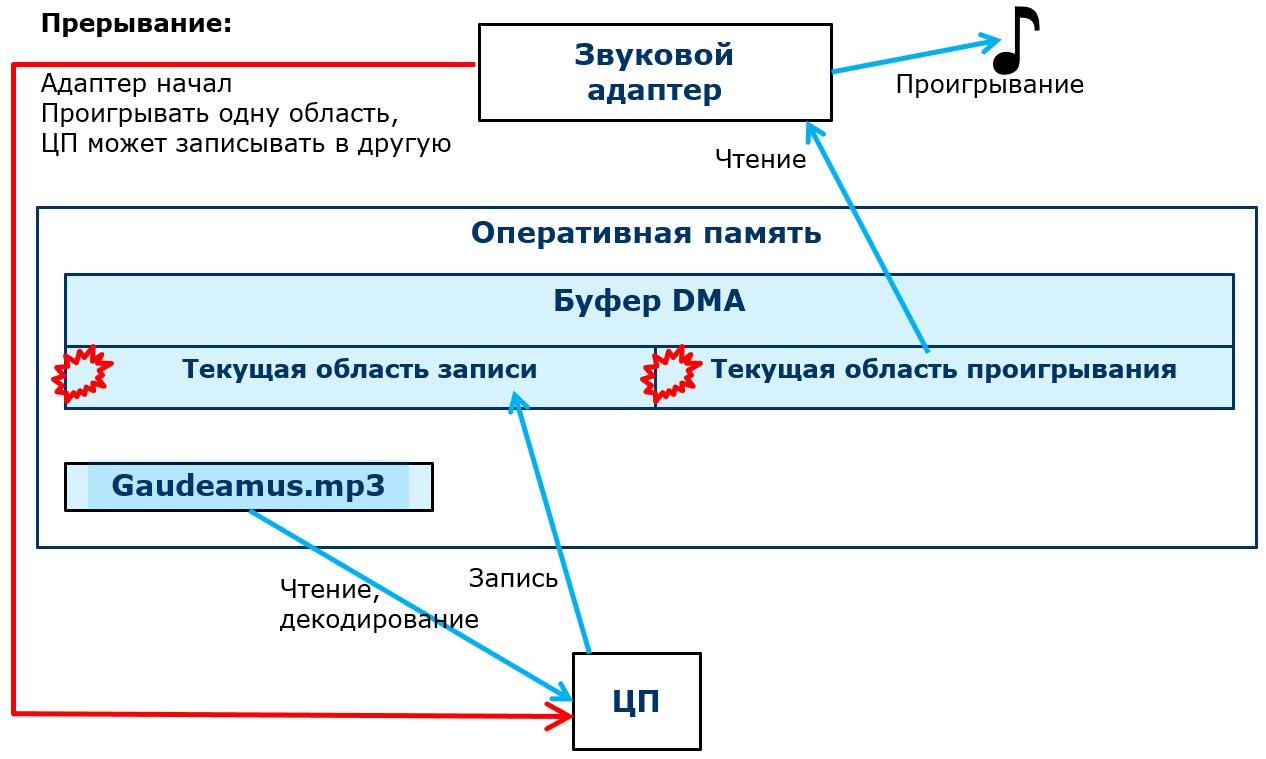
\includegraphics[height=0.65\textheight]{img/03.interrupt_DMA.png}
    \end{figure}

\end{frame}

\section{Настройка устройств}

\begin{frame}{Как настраивалось оборудование до середины 1990-х?}
	Классический способ --- jumpers, DIP switches

	\begin{figure}
		\centering
		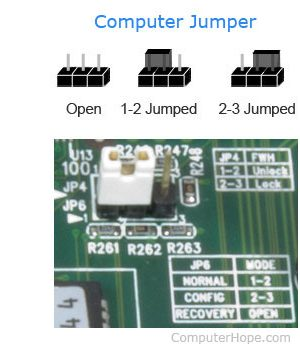
\includegraphics[height=0.5\textheight]{img/03.jumper.jpg}
	\end{figure}

	Настраивались \emph{системные ресурсы} --- адреса портов, характеристики DMA, номера аппаратных прерываний. Пример Sound Blaster для DOS: Port 220, IRQ 7, DMA 1
\end{frame}

\begin{frame}[fragile]{Как настраивается оборудование сейчас?}
	\begin{itemize}
		\item
		С середины 1980-х --- разные технологии для передачи метаданных по
		системной шине
		\item
		Первая широко внедрённая --- Plug-n-Play. Первая широко использующая            ОС для PC --- Windows 95 (жаргон конца 1990-х --- Plug and Pray)
	\end{itemize}

	\pause

	Посмотреть, какие ресурсы выделены устройствам в популярных ОС можно:

	\begin{itemize}
		\item
		В Windows --- при помощи Диспетчера устройств
		\item
		В Linux --- при помощи \mintinline{sh}{lsdev} (собирает информацию из
		\mintinline{sh}{/proc/interrupts}, \mintinline{sh}{/proc/ioports} и
		\mintinline{sh}{/proc/dma})
	\end{itemize}
\end{frame}

\section{Современные многоуровневые шины}

\begin{frame}{Зачем и почему?}
	TODO
\end{frame}

\subsection{PCI}

\begin{frame}{PCI, северный и южный мосты}
	TODO
\end{frame}

\subsection{PCI Express}

\begin{frame}{Зачем нужны асинхронные последовательные шины}
	TODO
\end{frame}

\begin{frame}{Root Complex, полосы}
	TODO
\end{frame}

\begin{frame}{Совместимость разъёмов разной ширины}
	TODO
\end{frame}


\section*{}

\begin{frame}{Упражнения и вопросы}
	\begin{block}{Упражнения}
		\begin{itemize}
			\tightlist
			\item
			Выберите несколько внутренних контроллеров своего ПК, выясните, какие
			системные ресурсы им выделены
            \item
            Идентифицируйте внутренние разъёмы расширения системной платы своего ПК
		\end{itemize}
	\end{block}

	\begin{block}{Вопросы}
		\begin{itemize}
			\tightlist
			\item
			Что такое аппаратное прерывание?
			\item
			Что такое драйвер, контроллер и порт?
			\item
			Что такое вектор и обработчик прерываний?
			\item
			Опишите принцип работы механизма DMA
			\item
			Каковы особенности DMA для устройств реального времени?
            \item
            В чём смысл использования последовательных шин расширения?
            \item
            Что такое северный и южный мосты?
            \item
            Что такое Root Complex?
		\end{itemize}
	\end{block}
\end{frame}

\postamble
\end{document}
